\chapter{Was bedeutet \textit{"reactive"} im Kontext der Softwareentwicklung}\label{was_ist_reactive_programming}
Grundlegend wird etwas als reaktiv bezeichnet, wenn eine Reaktion durch eine vorangegangene Aktion ausgelöst wird. Bei diesen Aktionen handelt es sich entweder um Veränderungen an verwendeten Daten oder stattfindende Ereignisse(\textit{Events}). Eine Beispiel zur Veranschaulichung ist die Benutzeroberfläche(\textit{GUI - Graphical User Interface}). Ein Benutzer bestätigt eine vorgenommene Eingabe durch das klicken eines Button innerhalb der GUI. Dieses Event sorgt dafür, dass die Applikation einen vorgegebenen Vorgang ausführt. Dieses Vorgehen sorgt in der klassischen objektorientierten Programmierweise mit sequentiellem Ablauf sowie dem imperativen Ansatz grundsätzlich für ein stetig wachsendes Maß an Komplexität. Durch die unterschiedlichen Events die innerhalb der GUI ausgelöst werden können(Mausklick, Tastendruck, usw.) ist ein klassisch imperativer und sequentieller Ablauf des Programmcodes nicht realistisch, da kein Entwickler weiß, in welcher Reihenfolge und zu welchem Zeitpunkt ein, beziehungsweise welches, Event ausgelöst wird.
\lstinputlisting[linerange={6-14}, float=hbt, caption={Implementierung des eigentlichen Event Handlers}, label=lst:handler]{../SystemMonitor/examples/eventhandling/Handler.java}
 Somit spielt hier die \textit{Inversion of Control}, also das Umkehren der Kontrolle, eine große Rolle \cite{MartinFowler.2005}. Diese besagt, dass nicht der programmierte Code den Ablauf beschreibt, sondern die Kontrolle bei dem Framework, welches für die Interaktion zuständig ist, liegt, und dieses entscheidet wiederum wie und wann auf ein Event reagiert wird. Im Code spiegelt es sich dadurch wider, dass mögliche Reaktionen, meist als Methoden oder Funktionen realisiert, an die mögliche eintreffenden Ereignisse gebunden werden. Dies geschieht über so genannte Event-Handler. \\
Im Listing \ref{lst:handler} sieht man eine Klasse welche das Event Hander Interface implementiert. Dieses Interface liefert eine Funktion \textit{handle(Event)} die implementiert werden muss. Innerhalb dieser Methode wird die Reaktion auf das aufgetretene Event definiert, in diesem Beispiel soll die Art des Events auf der Konsole ausgegeben werden. In Listing \ref{lst:eventrunner} wird nun dem einzigen Element der GUI, dem Button, ein Event Handler zugewiesen. Die Parameter besagen, dass jedes auftretenden Mouse-Event den Handler auslöst. Somit wird der Handler an ein auftretendes Ereignis gebunden, und der Programmablauf findet nicht mehr sequentiell statt, sondern das Framework der Oberfläche erkennt das Event und der passende Handler wird aufgerufen. An ein Objekt können mehrere Handler gebunden werden, die auf das gleiche oder unterschiedliche Events reagieren.

\lstinputlisting[linerange={10-29}, float=hbt, caption={Klasse zum Anwendungsstart in welcher auch der EventHander gesetzt wird.}, label=lst:eventrunner]{../SystemMonitor/examples/eventhandling/ApplicationRunner.java}
Die Abbildung \ref{pic:buttonapp} zeigt nun den Button an welchem der Event-Handler registriert wurde. Jedes Mouse-Event welches vom Button erkannt wird, löst diesen Handler aus. Eine Beispielausgabe sieht man in Abbildung \ref{pic:consoleoutput}. \\ Dieses Beispiel veranschaulicht wie grundsätzlich ein reaktives Verhalten einer Anwendung erzeugt wird. Es wird klar, dass Reaktivität somit schon lange in der Softwareentwicklung eine Rolle spielt.
\begin{figure}[hbt]
	\centering
	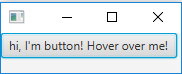
\includegraphics[width=0.4\textwidth]{Abb/buttonapp.PNG}
	\caption{Anwendung mit Button.}
	\label{pic:buttonapp}
\end{figure}
\begin{figure}[htb]
	\centering
	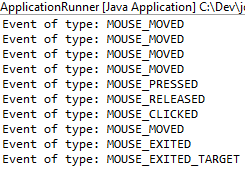
\includegraphics[width=0.4\textwidth]{Abb/consoleoutput.PNG}
	\caption{Die Konsolenausgabe für die Button Events.}
	\label{pic:consoleoutput}
\end{figure}
